\chapter{Algunos Teoremas}%
\label{cap:ejemplos}

\section{Teoremas y demostraciones}%
\label{sec:etiquetas}

Todos los ambientes que se desee referir por n\'umero m\'as adelante deben de
tener una etiqueta.  Consideremos por ejemplo el siguiente lema.

\begin{teorema}%
\label{teo:primero}
Sea $G$ una gr\'afica conexa con di\'ametro $d$. Entonces, $F_{k}(G)$ es 
conexa con di\'ametro al menos $k(d -k+1)$ y a lo m\'as $d k$.
\end{teorema}

\begin{proof}
Sean $A$ y $B$ v\'ertices de $F_{k}(G)$. Primero nos enfocamos en la cota
superior. Por definici\'on tenemos que $|A \triangle B| \leq |A \cup B|$, con
igualdad cuando $A \cap B = \varnothing$. Observamos que, al ser $A$ y $B$
v\'ertices de $F_{k}(G)$, tenemos que $|A|=k$ y $|B|=k$ por lo que $|A \cup B|
\le 2k$. Entonces, tenemos que $|A \triangle B| \leq 2k$, por lo que
$\frac{1}{2} |A \triangle B| \leq k$.

Buscamos demostrar que el di\'ametro de $F_{k}(G)$ es a lo m\'as $d k$, por
lo que basta demostrar, por inducci\'on, que para cualesquiera dos v\'ertices
$A$ y $B$ de $F_{k}(G)$ hay una $AB$-trayectoria de a lo m\'as
$\frac{d}{2}|A\triangle B|$. Observamos que esto tambi\'en implica que
$F_{k}(G)$ es conexa.

Si $A\triangle B=\varnothing$, entonces $A=B$ por lo que no hay nada que probar.
Ahora consideramos $A$ y $B$ tales que $A\triangle B \neq \varnothing$. Tomamos
como hip\'otesis que para cualesquiera dos v\'ertices de $F_{k}(G)$, $C$ y $D$,
tales que $|C\triangle D|<|A \triangle B|$, existe una $CD$-trayectoria con
longitud a lo m\'as $\frac{d}{2}|C\triangle D|$. Al tomar $A\triangle B
\neq \varnothing$ tenemos un v\'ertice de $G$ en $A\setminus B$ y un v\'ertice
en $B\setminus A$, que denotamos $a$ y $b$ respectivamente. Dado que el
di\'ametro de $G$ es $d$, entonces hay una $ab$-trayectoria de longitud a
lo m\'as $d$, digamos $P$.

Definimos $A'=(A\setminus \{a\})\cup \{b\}$ y la trayectoria $A\xrightarrow[P]{}
A'$ en $F_{k}(G)$. Observamos que, por un lado $b\in B\cap A'$ y $b\notin B\cap
A$, pero $b\in A\cup B$. Por otro lado tenemos que $a\notin A'$ por lo que
$a\notin A'\cup B$ y $a\notin A\cap B$, pero $a\in A\cup B$. Entonces, tenemos
que $a,b \in A\triangle B$ y $a,b \notin A'\triangle B$. Ahora tomamos $v\in A$
tal que $v \neq a$. Entonces, tenemos que $v \in A\triangle B$ si y s\'olo si
$v\in A'\triangle B$. Por lo tanto tenemos que $|A'\triangle B|=|A \triangle B|-
2$. Por hip\'otesis inductiva, sabemos que hay una $A'B$-trayectoria en
$F_{k}(G)$ de longitud a lo m\'as $\frac{d}{2}|A'\triangle B|$, que como se
observ\'o anteriormente, coincide con $\frac{d}{2}|A\triangle B| - d$.

Sabemos que $A\xrightarrow[P]{} A'$ tiene la misma longitud que $P$, que es a lo
m\'as $d$. Entonces, tenemos una $AB$-trayectoria de la forma $A\rightarrow
A'\rightarrow B$ que tiene longitud a lo m\'as $\frac{d}{2}|A\triangle
B|-d +d =\frac{d}{2}|A\triangle B|$. Por lo tanto tenemos que
$F_{k}(G)$ es conexa y tiene di\'ametro a lo m\'as $d k$.

Ahora demostraremos la cota inferior. Sabemos que $G$ es una gr\'afica conexa
con di\'ametro $d$, por lo que existen vertices que est\'an a distancia
$d$, digamos $x$ y $y$. Ahora construimos una partici\'on de $V$ usando  la
distancia que tiene cada v\'ertice a $x$. Es decir, para cada $i\in [0,d]$,
sea $V_{i}$ el conjunto de v\'ertices de $G$ a distancia $i$ de $x$. Entonces,
tenemos que $V_{0}=\{x\}$ y $y\in V_{d}$. Denotamos $d_x(v)$ a la distancia
entre $x$ y el v\'ertice $v$.

Sea $a$ el m\'\i{}nimo \'\i{}ndice para el cu\'al se tiene $k \leq |V_{0}\cup
V_{1}\cup \dots \cup V_{a}|$ y sea $b$ el m\'aximo \'\i{}ndice para el cu\'al se
tiene $k\leq |V_{b}\cup V_{b+1}\cup \dots \cup V_{d}|$. Tomamos $A$ un
$k$-\textit{subconjunto} de $V_{0}\cup \dots \cup V_{a}$  tal que $A\subseteq
V_{0}$ o $V_{0}\cup \dots V_{a-1}\subseteq A$. Tomamos $B$ un
$k$-\textit{subconjunto} de $V_{b}\cup \dots \cup V_{d}$ tale que
$B\subseteq V_{d}$ o $V_{b+1}\cup \dots \cup V_{d}$. 

Consideramos cualquier trayectoria entre $A$ y $B$ en $F_{k}(G)$. Cualquier
ficha inicialmente en $A$, digamos en el v\'ertice $v$ de $G$, se mueve a
alg\'un v\'ertice en $B$, digamos el v\'ertice $v'$ de $G$. Observamos que todas
las aristas de $G$ est\'an dentro de alg\'un $V_{i}$ o a lo m\'as entre alg\'un
$V_{i}$ y $V_{i+1}$, con $i\in[0,d]$. Entonces, para la ficha en $v$ se
necesitan al menos $d_x(v')-d_x(v)$ movimientos para llegar a $v'$, ocupando
s\'olo las aristas entre $V_{i}$ y $V_{i+1}$, $i\in [0,d]$. Por lo tanto,
el di\'ametro de $F_{k}(G)$ es al menos $\sum_{v\in A}(d_x(v')-d_x(v))=
\sum_{w\in B}d_x(w)-\sum_{v\in A}d_x(v)$. Observamos que, al ser $G$ conexa,
toda $V_{i}$ tiene al menos un elemento y por construcci\'on $V_{i} \cap
V_{i+1}=\varnothing$, para toda $i\in [0,d]$. Tomamos el caso en el que
$|V_{i}|=1$ para toda $i\in [0,d]$. Entonces, tenemos que $k\leq
|V_{b}\cup\dots\cup V_{d}|=|V_{b}|+|V_{b+1}|+\cdots +|V_d|$
$=\sum_{b}^{d}1 = d -b+1$. An\'alogamente tenemos que $k\leq
|V_{0}\cup V_{1}\cup \dots V_{a}|=|V_{0}|+|V_{1}|+\cdots + |V_{a}|$
$=\sum_{0}^{a} 1 = a+1$ En ambos casos la cota m\'\i{}nima se alcanza en la
igualdad, por lo que tomamos $a=k-1$ y $b=d-k+1$. Por lo tanto tenemos que
el di\'ametro de $F_{k}(G)$ es al menos $\sum_{j=d -k+1}^{d}j -
\sum_{i=0}^{k-1}i = k(d-k+1)$.
\end{proof}


\begin{lema}%
\label{lem:primero}
Sea $A$ un $k$-conjunto en la gr\'afica $G$ y $a, b \in V(G)$ tales que $a \in
A$ y $b \notin A$. Sea $A' = (A \setminus \{ a \}) \cup \{ b \}$. Si $P$ y $Q$
son $ab$-trayectorias internamente ajenas en $G$, entonces $A \xrightarrow[P]{}
A'$ y $A \xrightarrow[Q]{} A'$ son trayectorias internamente ajenas en
$F_{k}(G)$.
\end{lema}

\begin{proof}
    Primero, supongamos que $|V(P) \cap A| \geq 2$, con $V(P) \cap A = \{v_{1},
    v_{2}, \dots , v_{p}\}$, con $v_{1} = a$. Notemos que, si $k > p$, entonces
    $k-p$ fichas no est\'an sobre $P$, por lo que est\'an est\'aticas en todos
    los v\'ertices de $A \xrightarrow[P]{} A'$. Ahora, consideremos $R$ un
    v\'ertice interno de $A \xrightarrow[P]{} A'$. Por la observaci\'on anterior
    tenemos que  $|R \cap V(P)| = p$. Por construcci\'on de $A \xrightarrow[P]{}
    A'$, $R$ tiene una ficha en la trayectoria $(v_{p},b ]$. Entonces, $R$ no
    contiene al conjunto $\{v_{2}, \dots, v_{p}\}$. Por otro lado, como
    $\{v_{2}, \dots, v_{p}\}$ est\'a en $A \cap V(P)$, y $Q$ y $P$ son
    internamente ajenas, entonces $\{v_{2}, \dots, v_{p}\}$ est\'an est\'aticos
    en cada v\'ertice de $A \xrightarrow[Q]{} A'$. Por lo tanto tenemos que $A
    \xrightarrow[P]{} A'$ y $A \xrightarrow[Q]{}A'$ son trayectorias
    internamente ajenas. Al suponer que $|A \cap Q| \geq 2$, tenemos un caso
    an\'alogo al anterior.

    Ahora, supongamos que $|A \cap V(P)| = 1$ y $|A \cap V(Q)| = 1$, es decir,
    $A \cap V(P) = \{a\} = A \cap V(Q)$. Sin p\'erdida de generalidad suponemos
    que $P$ no es la arista $ab$. Entonces, tenemos que $P \setminus \{a,b\}
    \neq \varnothing$. Por lo tanto, tenemos que todo v\'ertice interno de $A
    \xrightarrow[P]{} A'$ tiene alg\'un v\'ertice de $P \setminus \{a, b\}$. Por
    otro lado, ya que $P$ y $Q$ son internamente ajenos y s\'olo comparten el
    v\'ertice $a$ con $A$, ning\'un v\'ertice interno de $A \xrightarrow[Q]{}
    A'$ tiene un v\'ertice de $P \setminus \{a, b\}$. Luego, cada v\'ertice
    interno de ambas trayectorias tiene intersecci\'on vac\'\i{}a con $A$.
    Concluimos que $A \xrightarrow[P]{} A'$ y $A \xrightarrow[Q]{} A'$ son
    internamente ajenas.
\end{proof}

\begin{lema}%
\label{lem:segundo}
    Sea $H$ una gr\'afica bipartita completa con clases de color $Y$ y $Z$,
    donde $|Y|<|Z|$. Si las aristas de $H$ est\'an coloreadas de azul y rojo de
    manera que cada v\'ertice de $Y$ es incidente en a lo m\'as una arista roja,
    entonces $H$ tiene un conjunto $M$ de aristas azules tal que cada v\'ertice
    en $Y$ incide en exactamente una arista de $M$. Adem\'as, la uni\'on de
    aristas rojas y aristas de $M$ es ac\'\i{}clica.
\end{lema}

\begin{proof}
    Sea $H$ una gr\'afica bipartita completa con clases de color $Y$ y $Z$ como
    se especificaron. Demostramos el resultado por inducci\'on sobre $|Y|$. 

    Primero, supongamos que $Y=\{y\}$. Como $H$ es bipartita completa, existe
    una arista azul $e$ tal que $y$ es incidente en $e$.   Sea $M = \{ e \}$.
    Por otro lado, a lo m\'as existe una arista roja incidente en $y$, digamos
    $e'$. Entonces la uni\'on de aristas rojas y aristas en $M$ es $\{e, e'\}$,
    que no es un ciclo.

    Ahora supongamos que $|Y|>1$. Como tenemos que $|Y|<|Z|$, y hay a lo m\'as
    una arista roja incidente en cada v\'ertice de $Y$, entonces existe alg\'un
    $x \in Z$ tal que no tiene aristas rojas incidentes. Sea $v \in Y$ y sea
    $e$, en caso de existir, la arista roja incidente en $v$. Tomamos $H'=
    (H-v)-x$ con $R'$ el conjunto de aristas rojas de $H'$. Observamos que $Y' =
    Y- v$ y $Z'= Z- x$ son las clases de color de $H'$. Por hip\'otesis de
    inducci\'on, existe un conjunto $M'$ de aristas azules incidentes en $H'$
    tal que cada v\'ertice de $Y'$ incide exactamente en una arista de $M'$.
    Adem\'as $R'\cup M'$ es ac\'\i{}clico.
    
    En $H$, definimos $M = M'\cup \{xv\}$. Al tomar $x$ sin aristas rojas
    tenemos que $M$ cumple tener una arista azul por v\'ertice en $Y$. Tambi\'en
    definimos $R= R'\cup \{ e \}$, si es que existe $e$.  Dado que  $M'\cup R'$
    es ac\'\i{}clica y las aristas $\{vx\}$ y $e$, en caso de existir, no
    est\'an en $M'\cup R'$, entonces tenemos que $M \cup R$ es ac\'\i{}clica.
\end{proof}

\begin{lema}%
\label{lem:tercero}
    Sea $G$ una gr\'afica $t$-conexa. Sean $A$ y $B$ v\'ertices de $F_{k}(G)$
    tales que $|A \triangle B| = 2$. Entonces hay $t$ $AB$-trayectorias
    internamente ajenas en $F_{k}(G)$. Adem\'as, si $t \geq k$, entonces hay
    $k(t- k + 1)$ $AB$-trayectorias internamente ajenas en $F_{k}(G)$.
\end{lema}

\begin{proof}
    Sea $G$ una gr\'afica $t$-conexa y sean $A$ y $B$ v\'ertices de $F_{k}(G)$
    tales que $|A \triangle B| = 2$. Primero buscamos probar el n\'umero de
    $AB$-trayectorias internamente ajenas en $F_{k}(G)$ es al menos $t$. 
    
    Sean $a \in A \setminus B$ y $b \in B \setminus A$ los v\'ertices en la
    diferencia sim\'etrica. Al ser $G$ una gr\'afica $t$-conexa, entonces por el
    Teorema General de Menger, existen $P_{1}, \dots, P_{t}$ $ab$-trayectorias
    internamente ajenas en $G$. Por lo tanto, por el Lema 1.1.2, existen $A
    \xrightarrow[P_1]{}  B, \dots, A \xrightarrow[P_t]{}  B$ $AB$-trayectorias
    internamente ajenas en $F_{k}(G)$. 

    Ahora buscamos demostrar que, si $t \geq k$, entonces el n\'umero de
    $AB$-trayectorias internamente ajenas en $F_{k}(G)$ es al menos $k(t- k
    +1)$. Si $t=k$, entonces tenemos que $k(t - k + 1) = t(t-t+1) = t$ por lo
    que tenemos el caso anterior. Por lo tanto consideramos  $t \geq k + 1$. Sea
    $\mathcal{P}$ un conjunto m\'aximo de $ab$-trayectorias internamente ajenas
    en $G$. Por el Teorema General de Menger sabemos que $|\mathcal{P}| \ge t$.
    Elegimos un conjunto $\mathcal{P}$ para el que ninguna trayectoria tenga
    cuerdas. Definimos a las trayectorias $P_{1}, \dots, P_{l}$ como aquellas en
    $\mathcal{P}$ que no intersectan a $A \cap B$ y $Q_{1}, \dots, Q_{s}$ las
    trayectorias en $\mathcal{P}$ que intersectan a $A \cap B$. Entonces $l + s
    = |\mathcal{P}| \ge t$.

    Definimos a $C$ como el conjunto de v\'ertices en $A \cap B$ que intersectan
    alg\'un $Q_i$, con $i \in \{1, \dots, s\}$. Observamos que, al ser $Q_1,
    \dots, Q_s$ internamente ajenos, entonces cada v\'ertice de $C$ esta en
    exactamente un $Q_i$, con $i \in \{1, \dots, s\}$. 

    Definimos $D$ como el conjunto de v\'ertices en $A \cap B$ que no intersecta
    a ning\'un $Q_i$, con $i \in \{1, \dots, s\}$. Observamos que $C$ y $D$
    dividen a $A \cap B$. Entonces, tenemos que $|A\cap B| = |C| + |D| = k-1$.
    Adem\'as podemos ver que $s \leq |C| \leq k-1$ y como $ t - s \leq l$,
    entonces $l \geq t -|C| = t- (k-1-|D|)$.

    Podemos separar las $AB$-trayectorias construidas en $F_{k}(G)$ en tres
    tipos. Los primeros dos tipos son las trayectorias obtenidas del Lema 1.1.2,
    es decir, las trayectorias $A \xrightarrow[P_1]{}  B, \dots, A
    \xrightarrow[P_l]{}  B$ y $A \xrightarrow[Q_1]{}  B, \dots, A
    \xrightarrow[Q_s]{}  B$. Nombramos a estos tipos de $AB$-trayectorias
    trayectorias de tipo $P$ y de tipo $Q$ respectivamente. Notamos que, por
    como se defini\'o, toda $AB$-trayectoria de tipo $P$ no pasa por $A\cap B$,
    por lo que cada trayectoria de este tipo corresponde a la sequencia de
    fichas obtenidas al mover la ficha de $a$ a trav\'es de $P_i$ hacia $b$, con
    $i \in \{1, \dots, l\}$.
    
    Ahora construimos las trayectorias de tipo $R$ utilizando los vecinos de $v
    \in A \cap B$. Primero consideramos $v \in C$, por lo que $v \in Q_i$ para
    un  $i \in \{1, \dots, s\}$. Definimos $Y_v = N_G(v) \setminus ((A \cap B)
    \cup Q_i)$. Dado que $G$ es una gr\'afica $t$-conexa, $|Y_v| = d_G(v) \geq
    t$. A su vez, $|A \cup B| =k -1$ y $v \in (A \cap B) \setminus N_G(v)$. Por
    \'ultimo, como $Q_i$ no tiene cuerdas, $v$ s\'olo tiene dos vecinos en
    $Q_i$. Por lo tanto tenemos que $|Y_v| \geq t- (k-2)-2 = t-k$. 
    
    Consideramos $v \in D$ y definimos $Y_v = N_g(v) \setminus (A \cup
    B)$. Al ser $G$ una gr\'afica $t$-conexa, se cumple $|N_G(v)| = d_G(v) \geq
    t$. Adem\'as tenemos que $|A \cup B| = k + 1$ y $v \in (A \cup B) \setminus
    N_G(v)$. Ahora, notemos que $(a, v, b)$ no es una trayectoria en $G$. \'Esto
    pues de lo contrario tendr\'i{}amos una trayectoria cuyo \'unico v\'ertice
    interno no est\'a en ning\'un $P_i$ y ning\'un $Q_j$, con $i \in \{1, \dots,
    l\}$ y $j \in \{1, \dots, s\}$, por lo que la trayectoria no estar\'i{}a en
    $\mathcal{P}$. Por lo que concluimos que $A \notin N_G(v)$ o $b \notin
    N_G(v)$. Por lo tanto tenemos que $|Y_v| \geq t- (k-1) = t-k + 1$.

    Nombramos $Y_v '$ al subconjunto de $Y_v$ con cardinalidad m\'i{}nima, es
    decir, $|Y_v '| = t-k$ si $v \in C$ y $|Y_v '| = t- k+ 1$ si $v \in D$.
    Notamos que $Y_v ' \neq \varnothing$ porque tomamos $t \geq k + 1$, adem\'as
    tenemos que $a, b \notin Y_v '$ por definici\'on. 

    Sea $H_v$ la gr\'afica bipartita completa con clases de colores $Y_v '$ y
    $\{1,\dots, l\}$. Definimos la siguiente coloraci\'on, si $y \in P_i$, para
    alg\'un $i \in \{1, \dots, l\} y y \in Y_v '$, entonces coloreamos la arista
    $iy$ de rojo. Coloreamos el resto de las aristas de la gr\'afica de azul.
    
    Ahora veamos si la coloraci\'on definida cumple las hip\'otesis del
    Lema1.1.3. Primero tenemos que por construcci\'on de los $P_i$, con $i \in
    \{1, \dots, l\}$, cada v\'ertice de $Y_v '$ est\'a en a lo m\'as un $P_i$,
    por lo que cada v\'ertice de $Y_v '$ incide en a lo m\'as una arista roja.
    Luego, notemos que $|\{1, \dots, l\}| = l  \geq t-k+ 1+ |D| > t-k + |D|$. Si
    $v \in D$, entonces $|D| \geq 1$ por lo que $l \geq t- k+1 = |Y_v '|$. Si $v
    \in C$, tenemos que $l \geq t-k = |Y_v '|$. Entonces podemos usar el Lema
    1.1.3 en $H_v$ con $Z= \{1, \dots, l\}$ y $Y = Y_v '$. Por lo tanto hay un
    conjunto $M_v$ de aristas azules tal que cada v\'ertice en $Y$ incide en
    exactamente una arista de $M_v$ y la uni\'on de aristas rojas y aristas de
    $M_v$ es ac\'\i{}clica. Notamos que $|M_v|=|Y_v '|$.

    Usando la $M_v$ construimos las trayectorias de tipo $R$ de la siguiente
    manera. Para cada $jx \in M_v$ defininimos $R\langle v, x \rangle$ como la
    trayectoria en $F_k(G)$ que corresponde a mover la ficha en $v$ hacia $x$,
    luego recorrer la trayectoria $A\setminus \{v\} \xrightarrow[P_j]{}
    (A\setminus \{v\})'$ y por \'ultimo mover la ficha de $x$ hacia $v$. Notemos
    que las fichas en $(A\cap B)\setminus \{v\}$ estan estacionarias. Adem\'as,
    cada v\'ertice en $R\langle v,x \rangle$ se conforma por $((A\cap
    B)\setminus \{v\}) \cup \{x\}$ y alg\'un v\'ertice $y \in P_i$.


    Falta ver que cada trayectoria de tipo $R$ es internamente ajena al resto de
    las trayectorias. Primero veamos que las trayectorias de tipo $R$ son
    internamente ajenas dos a dos. Supongamos que existen $R \langle v, x
    \rangle$ y $R\langle v',x' \rangle$ tales que $(v,x) \neq (v',x')$ pero
    comparten un v\'ertice interno. Entonces tenemos que $ix \in M_v$ y $i'x'\in
    M_v'$, con $i, i' \in \{1, \dots, l\}$. Por construcci\'on de las
    trayectorias de tipo $R$ tenemos que $((A\cap B)\setminus \{v\}) \cup \{x,
    y\} =((A\cap B)\setminus \{v'\}) \cup \{x', y'\}$ para alg\'un $y \in P_i$ y
    $y' \in P_{i'}$. Al tener $x'\in Y_{v'} '$ tenemos que $x'\in \{x,y\}$, pues
    $((A \cap B )\setminus \{v\}) \cap Y_{v'}'= \varnothing$. An\'alogamente
    tenemos que $y'\in \{x, y\}$ ya que $(A \cap B) \cap P_i = \varnothing$. Por
    lo tanto tenemos $\{x,y\}= \{x',y'\}$, lo cual implica que $(A\cap
    B)\setminus \{v\} = (A\cap B)\setminus \{v'\}$, entonces $v = v'$. \'Esto
    implica que $ix, i'x' \in M_v$, pero por construcci\'on cada v\'ertice de
    $Y_v '$ es incidente en s\'olo una arista de $M_v$, por lo que $x \neq x'$ y
    $i \neq i'$. Como tenemos que $\{x, y\}=\{x', y'\}$, entonces $x=y'$ y
    $y=x'$. Entonces tenemos que $x \ in P_{i'}$ y $x'\in P_i$, lo cual implica
    que $xi'$ y $x'i$ son aristas rojas en $H_v$. Por lo tanto tenemos el ciclo
    $(x, i, x', i)$ con aristas de color azul, rojo, azul, rojo respectivamente,
    lo cual es una contradicci\'on. As\'i pues, las trayectorias de tipo $R$ son
    internamenta ajenas dos a dos.

    Ahora veamos que las trayectorias de tipo $R$ y las de tipo $P$ son
    internamente ajenas entre s\'i{}. Sean $R\langle v,x \rangle$ y $A
    \xrightarrow[P_i]{}  B$, para alg\'un $i \in \{1, \dots, l\}$, trayectorias
    en $F_k(G)$ de tipo $R$ y $P$ respectivamente. Por construcci\'on, $v$ no
    est\'a en ning\'un v\'ertice interno de $\langle v,x \rangle$. Por otro
    lado, como $ v \in A\cap B$, entonces $v$ est\'a est\'atico en $A
    \xrightarrow[P_i]{}  B$, es decir, $v$ est\'a en cada v\'ertice de la
    trayectoria. Por lo tanto tenemos que las trayectorias $R\langle v,x
    \rangle$ y $A \xrightarrow[P_i]{}  B$, para alg\'un $i \in \{1, \dots, l\}$,
    son internamente ajenas.

    Por \'ultimo, veamos que las trayectorias de tipo $Q$ y las de tipo $R$ son
    internamente ajenas entre s\'i{}. Sean $R\langle v,x \rangle$ y $A
    \xrightarrow[Q_i]{}  B$, para alg\'un $i \in \{1, \dots, s\}$, trayectorias
    en $F_k(G)$ de tipo $R$ y $Q$ respectivamente. Sea $jx$ arista en $M_v$, con
    $j \in \{1, \dots. l\}$, entonces $x \notin P_j$. Si tomamos $v \notin Q_i$,
    entonces $v$ est\'a est\'atico en $A \xrightarrow[Q_i]{} B$, es decir,
    est\'a en cada v\'ertice de la trayectoria. Por otro lado, por
    construcci\'on tenemos que $v$ no est\'a en los v\'ertices internos de $R
    \langle v, x \rangle$. Por lo tanto las trayectorias son internamente
    ajenas. Ahora consideramos el caso en el que $v \in Q_i$, es decir $v \in
    C$. Por como definimos $R \langle v,x \rangle$, $x$ es est\'a en cada
    v\'ertice interno de la trayectoria. Por otro lado, como $x \in Y_v'$ y por
    construcci\'on tenemos que $Y_v ' \cap ((A\cap B) \cup Q_i) = \varnothing$,
    entonces $x \notin ((A \cap B) \cup Q_i)$. Por definici\'on, cada v\'ertice
    de $A \xrightarrow[Q_i]{}  B$ est\'a contenido en $((A \cap B) \cup Q_i)$,
    entonces $x$ no esta en los v\'ertices internos de $A \xrightarrow[Q_i]{}
    B$. Porl lo tanto tenemos que las trayectorias $R\langle v,x \rangle$ y $A
    \xrightarrow[Q_i]{}  B$ son internamente ajenas.

    Tenemos que hay $l$ y $s$ trayectorias de tipo $P$ y $Q$ respectivamente.
    Adem\'as, para cada $v \in C$ hay $t-k$ trayectorias de tipo $R$ y para cada
    $v \in D$ hay $t-k+1$ trayectorias de tipo $R$. Entonces en $F_k(G)$ hay $l+
    s+ |C|(t-k)+ |D|(t-k +1) = l + s + (|C| + |D|)(t-k) + |D| = l + s +
    (|k-1)(t-k) + |D|$ trayectorias internamente ajenas. Despejando tenemos que
    $l + s + (k-1)(t-k) + |D| \geq t+ (k-1)(t-k) = k (t -k +1)$. Por lo tanto el
    n\'umero de $AB$- trayectorias en $F_k(G)$ es al menos $k(t-k+1)$.
\end {proof}

\tikzset{every picture/.style={line width=0.75pt}} %set default line width to 0.75pt        

    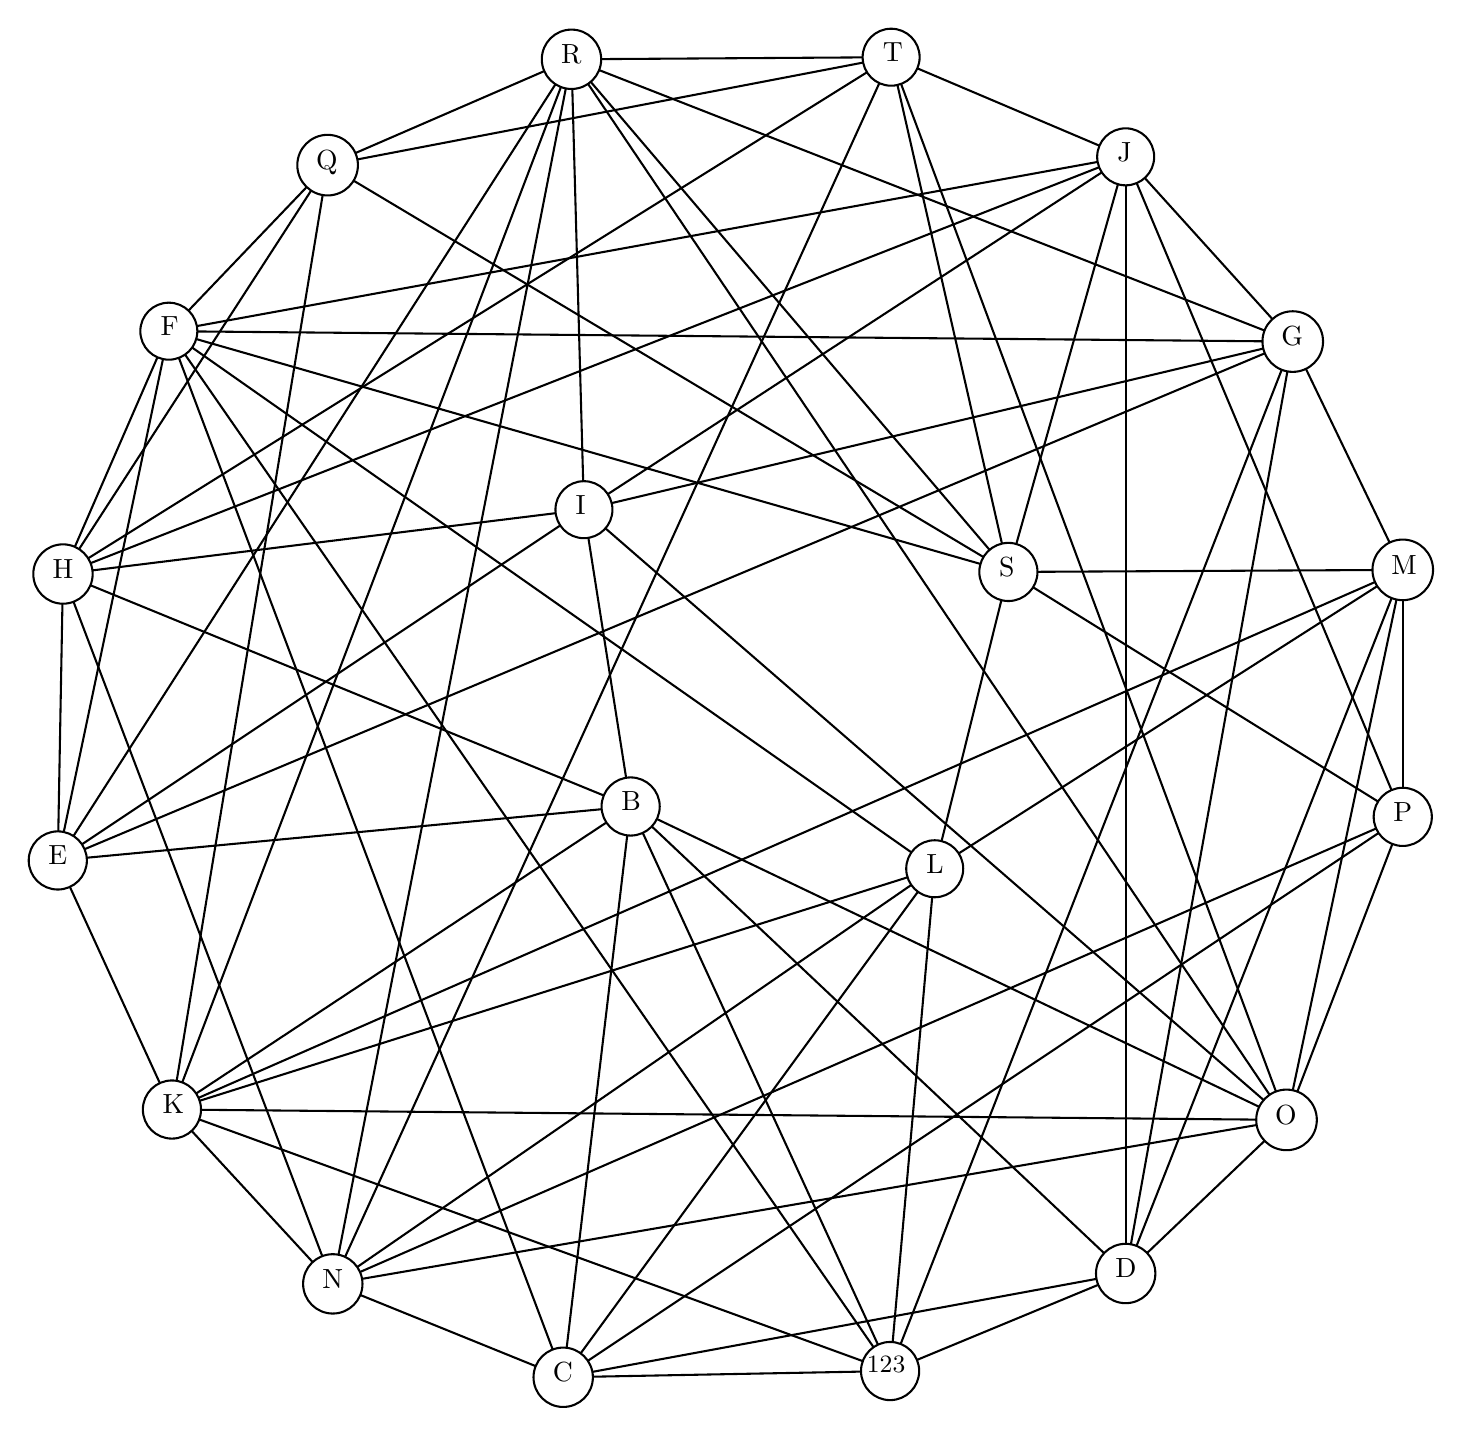
\begin{tikzpicture}[x=0.75pt,y=0.75pt,yscale=-1,xscale=1]
    %uncomment if require: \path (0,705); %set diagram left start at 0, and has height of 705
    
    
    % Text Node
    \draw    (407, 649.5) circle [x radius= 14.01, y radius= 14.01]   ;
    \draw (401,641) node [anchor=north west][inner sep=0.75pt]   [align=left] {\hspace{-5pt}{\small $123$}};
    % Text Node
    \draw    (282, 377.5) circle [x radius= 14.01, y radius= 14.01]   ;
    \draw (276,369) node [anchor=north west][inner sep=0.75pt]   [align=left] {B};
    % Text Node
    \draw    (61, 523.5) circle [x radius= 14.01, y radius= 14.01]   ;
    \draw (55,515) node [anchor=north west][inner sep=0.75pt]   [align=left] {K};
    % Text Node
    \draw    (249.5, 652.5) circle [x radius= 14.3, y radius= 14.3]   ;
    \draw (243,644) node [anchor=north west][inner sep=0.75pt]   [align=left] {C};
    % Text Node
    \draw    (59.5, 148.5) circle [x radius= 13.73, y radius= 13.73]   ;
    \draw (54,140) node [anchor=north west][inner sep=0.75pt]   [align=left] {F};
    % Text Node
    \draw    (428.5, 407.5) circle [x radius= 13.73, y radius= 13.73]   ;
    \draw (423,399) node [anchor=north west][inner sep=0.75pt]   [align=left] {L};
    % Text Node
    \draw    (601, 153.5) circle [x radius= 14.6, y radius= 14.6]   ;
    \draw (594,145) node [anchor=north west][inner sep=0.75pt]   [align=left] {G};
    % Text Node
    \draw    (520.5, 602.5) circle [x radius= 14.3, y radius= 14.3]   ;
    \draw (514,594) node [anchor=north west][inner sep=0.75pt]   [align=left] {D};
    % Text Node
    \draw    (6, 403.5) circle [x radius= 14.01, y radius= 14.01]   ;
    \draw (0,395) node [anchor=north west][inner sep=0.75pt]   [align=left] {E};
    % Text Node
    \draw    (8.5, 265.5) circle [x radius= 14.3, y radius= 14.3]   ;
    \draw (2,257) node [anchor=north west][inner sep=0.75pt]   [align=left] {H};
    % Text Node
    \draw    (259.5, 234.5) circle [x radius= 13.73, y radius= 13.73]   ;
    \draw (254,226) node [anchor=north west][inner sep=0.75pt]   [align=left] {I};
    % Text Node
    \draw    (520.5, 64.5) circle [x radius= 13.73, y radius= 13.73]   ;
    \draw (515,56) node [anchor=north west][inner sep=0.75pt]   [align=left] {J};
    % Text Node
    \draw    (654, 263.5) circle [x radius= 14.6, y radius= 14.6]   ;
    \draw (647,255) node [anchor=north west][inner sep=0.75pt]   [align=left] {M};
    % Text Node
    \draw    (138.5, 607.5) circle [x radius= 14.3, y radius= 14.3]   ;
    \draw (132,599) node [anchor=north west][inner sep=0.75pt]   [align=left] {N};
    % Text Node
    \draw    (598, 528.5) circle [x radius= 14.6, y radius= 14.6]   ;
    \draw (591,520) node [anchor=north west][inner sep=0.75pt]   [align=left] {O};
    % Text Node
    \draw    (654, 382.5) circle [x radius= 14.01, y radius= 14.01]   ;
    \draw (648,374) node [anchor=north west][inner sep=0.75pt]   [align=left] {P};
    % Text Node
    \draw    (136, 68.5) circle [x radius= 14.6, y radius= 14.6]   ;
    \draw (129,60) node [anchor=north west][inner sep=0.75pt]   [align=left] {Q};
    % Text Node
    \draw    (253.5, 17.5) circle [x radius= 14.3, y radius= 14.3]   ;
    \draw (247,9) node [anchor=north west][inner sep=0.75pt]   [align=left] {R};
    % Text Node
    \draw    (464, 264.5) circle [x radius= 14.01, y radius= 14.01]   ;
    \draw (458,256) node [anchor=north west][inner sep=0.75pt]   [align=left] {S};
    % Text Node
    \draw    (407.5, 16.5) circle [x radius= 13.73, y radius= 13.73]   ;
    \draw (402,8) node [anchor=north west][inner sep=0.75pt]   [align=left] {T};
    % Connection
    \draw    (401.15,636.77) -- (287.85,390.23) ;
    % Connection
    \draw    (393.83,644.71) -- (74.17,528.29) ;
    % Connection
    \draw    (392.99,649.77) -- (263.8,652.23) ;
    % Connection
    \draw    (399.02,637.99) -- (67.33,159.78) ;
    % Connection
    \draw    (408.24,635.55) -- (427.28,421.18) ;
    % Connection
    \draw    (412.1,636.45) -- (595.68,167.1) ;
    % Connection
    \draw    (419.95,644.14) -- (507.28,607.97) ;
    % Connection
    \draw    (268.05,378.81) -- (19.95,402.19) ;
    % Connection
    \draw    (269.03,372.19) -- (21.74,270.92) ;
    % Connection
    \draw    (270.31,385.22) -- (72.69,515.78) ;
    % Connection
    \draw    (280.36,391.41) -- (251.18,638.3) ;
    % Connection
    \draw    (292.19,387.11) -- (510.1,592.69) ;
    % Connection
    \draw    (294.64,383.54) -- (584.82,522.2) ;
    % Connection
    \draw    (236.24,647.13) -- (151.76,612.87) ;
    % Connection
    \draw    (244.45,639.12) -- (64.34,161.35) ;
    % Connection
    \draw    (257.94,640.95) -- (420.4,418.59) ;
    % Connection
    \draw    (261.4,644.56) -- (642.35,390.28) ;
    % Connection
    \draw    (263.57,649.9) -- (506.43,605.1) ;
    % Connection
    \draw    (530.84,592.62) -- (587.44,538.58) ;
    % Connection
    \draw    (520.5,588.2) -- (520.5,78.23) ;
    % Connection
    \draw    (523.02,588.42) -- (598.42,167.88) ;
    % Connection
    \draw    (525.74,589.19) -- (648.65,277.09) ;
    % Connection
    \draw    (11.84,416.24) -- (55.16,510.76) ;
    % Connection
    \draw    (6.25,389.49) -- (8.24,279.8) ;
    % Connection
    \draw    (13.56,391.71) -- (245.78,29.54) ;
    % Connection
    \draw    (17.66,395.73) -- (248.08,242.12) ;
    % Connection
    \draw    (18.92,398.07) -- (587.53,159.16) ;
    % Connection
    \draw    (8.88,389.79) -- (56.68,161.94) ;
    % Connection
    \draw    (54.01,161.09) -- (14.22,252.39) ;
    % Connection
    \draw    (70.74,156.39) -- (417.26,399.61) ;
    % Connection
    \draw    (72.7,152.29) -- (450.53,260.64) ;
    % Connection
    \draw    (73.23,148.63) -- (586.4,153.37) ;
    % Connection
    \draw    (73.01,146.04) -- (506.99,66.96) ;
    % Connection
    \draw    (68.99,138.58) -- (125.91,79.05) ;
    % Connection
    \draw    (607.34,166.66) -- (647.66,250.34) ;
    % Connection
    \draw    (591.2,142.67) -- (529.71,74.68) ;
    % Connection
    \draw    (587.4,148.18) -- (266.82,22.71) ;
    % Connection
    \draw    (586.79,156.87) -- (272.86,231.33) ;
    % Connection
    \draw    (16.27,253.49) -- (128.06,80.76) ;
    % Connection
    \draw    (20.63,257.93) -- (395.85,23.77) ;
    % Connection
    \draw    (21.81,260.27) -- (507.72,69.52) ;
    % Connection
    \draw    (22.69,263.75) -- (245.87,236.18) ;
    % Connection
    \draw    (261.63,248.06) -- (279.82,363.66) ;
    % Connection
    \draw    (269.87,243.5) -- (586.97,518.92) ;
    % Connection
    \draw    (259.12,220.78) -- (253.9,31.79) ;
    % Connection
    \draw    (271.01,227.01) -- (508.99,71.99) ;
    % Connection
    \draw    (507.86,59.13) -- (420.14,21.87) ;
    % Connection
    \draw    (516.77,77.72) -- (467.81,251.02) ;
    % Connection
    \draw    (525.82,77.16) -- (648.58,369.58) ;
    % Connection
    \draw    (70.5,533.8) -- (128.8,596.99) ;
    % Connection
    \draw    (13.58,278.87) -- (133.42,594.13) ;
    % Connection
    \draw    (63.28,509.68) -- (133.62,82.91) ;
    % Connection
    \draw    (65.98,510.4) -- (248.41,30.87) ;
    % Connection
    \draw    (74.36,519.28) -- (415.4,411.63) ;
    % Connection
    \draw    (73.83,517.87) -- (640.62,269.37) ;
    % Connection
    \draw    (75.01,523.63) -- (583.4,528.36) ;
    % Connection
    \draw    (431.81,394.17) -- (460.62,278.1) ;
    % Connection
    \draw    (417.2,415.3) -- (150.27,599.38) ;
    % Connection
    \draw    (440.07,400.11) -- (641.69,271.36) ;
    % Connection
    \draw    (654,278.1) -- (654,368.49) ;
    % Connection
    \draw    (650.98,277.79) -- (601.02,514.21) ;
    % Connection
    \draw    (639.4,263.58) -- (478.01,264.43) ;
    % Connection
    \draw    (152.6,605.08) -- (583.61,530.97) ;
    % Connection
    \draw    (151.61,601.78) -- (641.16,388.11) ;
    % Connection
    \draw    (144.43,594.48) -- (401.81,29) ;
    % Connection
    \draw    (141.24,593.46) -- (250.76,31.54) ;
    % Connection
    \draw    (603.23,514.86) -- (648.98,395.58) ;
    % Connection
    \draw    (592.91,514.81) -- (412.29,29.37) ;
    % Connection
    \draw    (589.84,516.39) -- (261.49,29.36) ;
    % Connection
    \draw    (642.1,375.11) -- (475.9,271.89) ;
    % Connection
    \draw    (149.4,62.68) -- (240.38,23.2) ;
    % Connection
    \draw    (150.35,65.75) -- (394.01,19.08) ;
    % Connection
    \draw    (148.54,75.99) -- (451.97,257.31) ;
    % Connection
    \draw    (267.8,17.41) -- (393.77,16.59) ;
    % Connection
    \draw    (262.78,28.38) -- (454.91,253.84) ;
    % Connection
    \draw    (460.89,250.84) -- (410.55,29.89) ;
    
    \end{tikzpicture}

\begin{teorema}%
\label{teo:segundo}
    Sea $G$ una gr\'afica $t$-conexa. Entonces $F_{k}(G)$ es $t$-conexa para
    todo $k>1$
\end{teorema}
        
\begin{proof}
Primero, observamos que $A$ y $B$ son v\'ertices adyacentes en $F_k(G)$ si y
s\'olo si $V(G) \setminus A$ y $V(G)\setminus B$ son adyacentes en $F_{n-k}(G)$.
Entonces tenemos que $F_k(G) \simeq F_{n-k}(G)$. Por lo tanto asumimos sin
p\'erdida de generalidad que $k \leq \frac{n}{2}$.

Sea $\mathcal{C}$ un m\'i{}nimo corte por v\'ertices de $F_k(G)$. Basta
demostrar que $|\mathcal{C}| \geq t$. Definimos $A$ y $B$ como los v\'ertices en
distintas componentes de $F_k(G)- \mathcal{C}$ tales que $|A \triangle B|$ es
m\'i{}nimo.

Si $|A \triangle B| = 2$, entonces por el Lema 1.1.4 tenemos que hay $t$
$AB$-trayectorias internamente ajenas en $F_k(G)$. Por lo que tenemos que
$|\mathcal{C}| \geq t$.

Ahora consideramos $|A \triangle B| = 2r \geq 4$. Definimos $A \setminus B
=\{a_1, \dots, a_r\}$ y $B \setminus A =\{b_1, \dots, b_r\}$. Tambi\'en
definimos $A_{i,x} = A\setminus \{a_i\} \cup \{x\}$ y $B_{j,x} = B\setminus
\{b_j\} \cup \{x\}$ para cada $i \in \{1, \dots, r\}$ y $x \in V(G)\setminus
(A\cup B)$. Supongamos que para algunos $i, j$ y $x$ tenemos que $A_{i,x} \notin
\mathcal{C}$ y $B_{j,x} \notin \mathcal{C}$. Como $A \triangle A_{i,x} = \{a_i,
x\}$, entonces tenemos que $|A \triangle A_{i,x}|< |A \triangle B|$ por lo que
$A$ y $A_{i,x}$ est\'an en la misma componente de $F_k(G)- \mathcal{C}$.
An\'alogamente tenemos que  $B$ y $B_{j,x}$ est\'an en la misma componente de
$F_k(G)-\mathcal{C}$

Luego nos fijamos en que $A_{i,x} \triangle B_{j,x} = (A \triangle B) \setminus
\{a_i, b_j\}$. Por lo que $|A_{i,x} \triangle B_{j,x}| = 2(r-1)$. As\'i{}
tenemos que $A_{i,x}$ y $B_{j,x}$ est\'an en la misma componente de $F_k(G)-
\mathcal{C}$. Pero tenemos que $A$ y$A_{i,x}$ est\'an en la misma componente, de
$F_K(G) - \mathcal{C}$, de igual manera que $B$ y $B_{j,x}$. Por lo tanto $A$ y
$B$ est\'an en la misma componente de $F_k(G)- \mathcal{C}$. Esto es una
cotradicci\'on pues tomamos a $A$ y $B$ en distintas componentes, lo que implica
que $A_{i,x}$ o $B_{j,x}$ est\'a en $\mathcal{C}$, para todas las $i,j$ y $x$.

Por lo anterior tenemos que, para cada $x \in V(G)\setminus (A \cup B)$,
$\mathcal{C}$ tiene todos los $\{A_i,x | i \in \{1, \dots, r\}\}$ o todos los
$\{B_j,x | j \in \{1, \dots, r\}\}$. Dado que $|A\cup B|=k +r$, sabemos que
$\mathcal{C}$ tiene al menos $r(n-k-r)$ v\'ertices.

Ahora definimos $A_{i,j} = (A\setminus \{a_i\}) \cup \{b_j\}$ y $B_{i,j} =
(B\setminus \{b_i\}) \cup \{a_j\}$, para toda $ i, j \in \{1, \dots, r\}$.
Notamos que hay $2r^2$ de estos conjuntos. Ahora supongamos que $A_{i,j} \notin
\mathcal{C}$, para algunos $ i, j \in \{1, \dots, r\}$. Entonces tenemos que $A
\triangle A_{i,j} = \{a_i, b_j\}$. Entonces $A$ y $A_{i,j}$ est\'an en la misma
componente de $F_k(G)- \mathcal{C}$. Por otro lado, $|B \triangle A_{i,j}| = 2
(r-1)$, por lo que $B$ y $A_{i,j}$ est\'an en la misma componente de $F_k(G) -
\mathcal{C}$. Por lo tanto tenemos que $A$ y $B$ est\'an en la misma componente
de $F_k(G)-\mathcal{C}$, lo cu\'al nos lleva a la misma contradicci\'on que el
caso anterior. Por lo tanto tenemos que $A_{i,j} \in \mathcal{C}$ para toda $i,
j \in \{1, \dots, r\}$. De manera an\'aloga $B_{i,j} \in \mathcal{C}$. Por lo
tanto tenemos que $\mathcal{C}$ tiene $2r^2$ v\'ertices, adem\'as de los del
caso anterior.

As\'i, tenemos que $|\mathcal{C}|\geq r(n-k-r)+2r^2 = r(n-k) + r^2$, pero $r
\geq 2$ y $k \leq \frac{n}{2}$, por lo que tenemos que $|\mathcal{C}| \geq
r(n-k)+r^2 > r(n-k) \geq 2(n-k) \geq n >t$. Por lo tanto $|\mathcal{C}|>t$.
\end{proof} 

\begin{teorema}%
    \label{teo:tercero}
        Sea $G$ una gr\'afica $t$-conexa con $t \ge k$ y $n \ge \frac{1}{2} kt$.
        Entonces $F_{k}(G)$ es $k (t- k+ 1)$-conexa.
    \end{teorema}

    \begin{proof}
        Sea $\mathcal{C}$ un corte por v\'ertices m\'i{}nimo de $F_k(G)$. Sean
        $A$ y $B$ v\'ertices en distintas componentes de $F_k(G)- \mathcal{C}$
        tales que $|A \triangle B|$ es m\'i{}nima.

        Si $|A \triangle B| = 2$, entonces por el Lema 1.1.4 tenemos que
        $F_k(G)$ tiene $k (t- k+ 1)$ $AB$-trayectorias. Por lo que tenemos que
        $|\mathcal{C}| \geq k (t- k+ 1)$.

        Ahora veamos el caso en el que $|A \triangle B| = 2r \ge 4$. Utilizando
        la desigualdad que se utiliza al final de la demostraci\'on
        d\cref{teo:segundo} tenemos que $|\mathcal{C}| \ge r(n-k-r)+2r^2$. Dado
        que $r \ge 2$ y $n \ge \frac{1}{2}kt$, entonces tenemos que
        $|\mathcal{C}| \ge r(n-k-r)+2r^2 \ge 2 (n- k -2) + 8 \ge tk - 2k+ 4$.
        Observamos que $k^2 -3k + 4 \ge 0$ para toda $k \ge 1$. Entonces tenemos
        que $-2k+4 \ge -k^2 + k$, esto implica que $kt -2k +4 \ge kt - k^2 + k =
        k (t - k +1)$. Entonces tenemos que $|\mathcal{C}| \ge tk -2k +4 \ge
        k(t-k+1)$. Por lo tanto $F_k(G)$ es $k(t-k+1)$-conexa.
    \end{proof}